Siguiendo la planificación expuesta en la sección \ref{roadmap}, la implementación se realiza de manera progresiva, centrando inicialmente los esfuerzos en el desarrollo de un prototipo. El objetivo es disponer lo antes posible de una versión de prueba del chatbot, publicarla y probarla  con un pequeño subconjunto de personas. Esto permite recopilar conversaciones reales de los usuarios y orientar el desarrollo hacia las necesidades detectadas. Durante este proceso, el asistente se irá nutriendo de información y mejorando hasta alcanzar un estado de madurez suficiente. Por tanto, tal y como se puede observar en la Figura \ref{fig:fasesApp}, a lo largo del desarrollo la aplicación irá evolucionando desde el prototipo inicial, pasando por una fase \textit{beta} hasta ser considerada como estable.\\  

\begin{figure}[htbp]
\centering
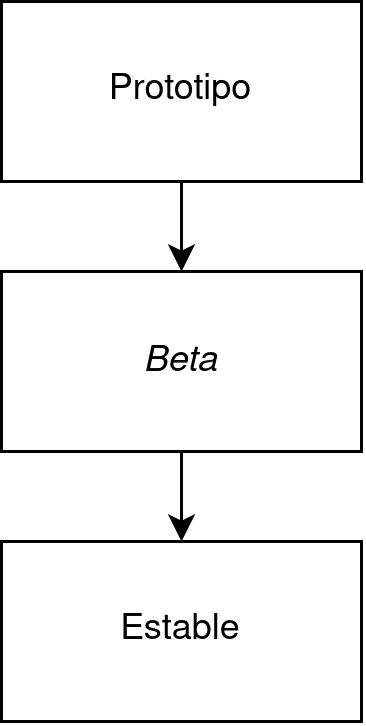
\includegraphics[scale=0.2]{../images/appStages.png}
\caption{Evolución de la aplicación}
\label{fig:fasesApp}
\end{figure}


A continuación, se procede a detallar los distintos pasos seguidos para llevar a cabo este proceso.\\


\subsection{Conjunto de entrenamiento inicial}
El conjunto de entrenamiento o \textit{dataset} hace referencia a los datos que se utilizan para entrenar un sistema conversacional en la tarea de reconocer las intenciones expresadas por los usuarios y en responder adecuadamente. En \textit{Rasa}, estos datos se estructuran mediante una serie de archivos en formato \textit{YAML} (\textit{YAML Ain't Markup Language}) que contienen las distintas entidades que representan una conversación. Así, los \textit{intents}  (intenciones) definen las diferentes preguntas que los usuarios pueden realizar, las respuestas contienen los mensajes que el chatbot devolverá y las \textit{stories} (historias) establecen los patrones de conversación. Con todos estos datos, posteriormente el asistente trata de identificar correctamente las intenciones expresadas por los usuarios y responder en consecuencia, según le haya sido indicado.\\

Para que el asistente pueda mantener conversaciones lo más amplias y variadas posibles, se han añadido al conjunto de entrenamiento \textit{intents}, respuestas y \textit{stories} pertenecientes a 3 áreas distintas: conocimiento médico, expresiones básicas y conversación informal. Los datos médicos están orientados a responder todas las dudas médicas sobre el VIH y han sido extraídos de la hoja de cálculo facilitada por parte de la Unidad de Enfermedades Infecciosas del Hospital General de Elche. Este documento consta de 130 preguntas con sus correspondientes respuestas y contiene todo el conocimiento médico que inicialmente tendrá el chatbot.\\

A parte de todas las cuestiones relacionadas con el VIH, el asistente debe ser también capaz de entender y desenvolverse con una serie de expresiones básicas que suelen formar parte un diálogo. Las conversaciones suelen empezar con un \textit{Hola} o \textit{¡Buenos días!} y suelen ser correspondidas con otro saludo, seguidas de un \textit{¿Cómo estás?} o \textit{¿Cómo va?} y sus correspondientes respuestas. Durante el transcurso, también pueden aparecer otras expresiones como afirmaciones o negaciones (\textit{¡Por supuesto!}, \textit{Claro}, \textit{Para nada} etc) o peticiones como \textit{¿Me puedes ayudar?} o \textit{Necesito tu ayuda}. Finalmente, se suele usar un \textit{Adiós} o \textit{Hasta luego} para despedirse y finalizar la conversación. Todas estas expresiones y muchas otras aparecen tarde o temprano en una conversación, y por tanto, se han incorporado el mayor numero posible de ellas al conjunto de entrenamiento para que el asistente las entienda y pueda hacer uso de ellas. En la la Figura \ref{fig:expresiones auxiliares} se muestra un ejemplo de una pequeña conversación donde se utilizan varias de estas expresiones.\\

\begin{figure}[htbp]
\centering

\includegraphics[scale=0.15]{../images/basics_chat.png}

\includegraphics[scale=0.15]{../images/basics_chat_2.png}
\caption{Ejemplo de una pequeña conversación}
\label{fig:expresiones auxiliares}
\end{figure}

Además, también es común que los usuarios intenten mantener un poco de conversación informal con el bot. Algunos de los ejemplos más repetidos como \textit{¿Cómo te llamas?}, \textit{Quién te ha creado?} o \textit{¿Qué tiempo hace?} han sido también incorporados al conjunto. A continuación se detalla para cada entidad el proceso que se ha seguido para incorporar la información al \textit{dataset}.\\

\subsubsection{\textit{Intents}}
Cada vez que escribimos un mensaje expresamos una intención. Los \textit{intents} representan y definen estas intenciones recopilando una gran cantidad de ejemplos reales. Es importante tener en cuenta que una determinada intención puede ser expresada de distintas maneras. Pongamos por caso la pregunta  \textit{¿Existe cura para el VIH?} extraída de la hoja de cálculo. La cuestión expresa la intención del usuario de querer saber si existe algún tratamiento que cure completamente el VIH. Sin embargo, esta es simplemente una  de las múltiples formas que existen de preguntarlo, pues sería igualmente posible formular \textit{¿Hay cura para el VIH?} o \textit{¿El VIH tiene cura?} expresando la misma intención.\\

Por tanto, un usuario puede expresar la misma intención a través de diferentes expresiones. Por ello, cada pregunta o expresión a la cuál que se quiera poder responder, se debe analizar para identificar la intención, y en base a esta, elaborar una serie de variaciones que garanticen un amplio espectro de reconocimiento.
Estas variaciones consisten en:

\begin{itemize}
	\item Reformulaciones parciales o completas de las preguntas.
	\item Variantes con faltas de ortografía.
	\item Variantes con errores de escritura.
\end{itemize}

En consecuencia, y siguiendo con el ejemplo anterior, para \textit{¿Existe cura para el VIH?} se pueden obtener diferentes variaciones como las siguientes:

\begin{verbatim}
- intent: cura_vih
  examples: |
    - ¿Existe cura para el VIH?
    - existe ya cura para el vih?
    - han inventado alguna cura para el vih?
    - que cura hay para el vih?
    - se puede sanar el vih?
    - es posible expulsar el virus del cuerpo?
    - es posible exulsar el vih?
    - tiene cura el sida?
    - como se cura elsida?
    - puede alguienr ecuperarse completamente del vih?
    - ...
\end{verbatim}

Es importante considerar que, para que posteriormente el modelo generado distinga de forma fiable una intención de otra, los ejemplos deben ser distintos entre los \textit{intents}. Es decir, no se debe utilizar el mismo ejemplo de entrenamiento para dos intenciones diferentes. Si los ejemplos de entrenamiento resultan demasiado similares, se produce una confusión de intenciones \cite{bestPracticesNLU}.\\ 

En esta fase inicial de la implementación, y siguiendo las recomendaciones de \textit{Rasa}, se generan manualmente 30 variaciones por cada intención. En total, se implementan 167 \textit{intents}, (133 acerca del VIH, 23 expresiones básicas y 11 de cháchara). Con esto se pretende garantizar unos resultados suficientemente satisfactorios para lanzar un primer prototipo. En las siguientes fases del desarrollo el número de variaciones aumentará con la recogida de datos reales (ver sección \ref{cdd}).\\

\subsubsection{Respuestas}
Las respuestas ofrecidas por el asistente son la pieza clave para formar y transmitir personalidad. En VIHrtual-App se ha querido crear y dotar al \textit{bot} de una personalidad propia implementando los rasgos comentados en la sección \ref{interaccion} \textit{Interacción y características sociales}.\\

Como ejemplo, a continuación se puede observar las posibles respuestas que el chatbot puede dar a un usuario que le pregunte \textit{¿Cómo estas?}. Al responder el chatbot escoge al azar una de las variantes, añadiendo cierto dinamismo a las contestaciones para intentar no transmitir la sensación robótica de los mensajes predefinidos. Además, los textos han sido construidas utilizando varios de los recursos mencionados anteriormente, como el uso de buenos modales, el tono algo informal y la proactividad. \\

\begin{verbatim}
  utter_estado:
    - text: Genial! ¿Tú que tal?
    - text: Genial, la verdad. Muchas gracias por preguntar.
    - text: Hoy me encuentro genial, ¡gracias por preguntar!
    - text: Hoy me siento especialmente bien. ¿Y tú que tal?
    - ...
\end{verbatim}

En el caso de las información médica, se detecta que las respuestas proporcionadas por el hospital son, en muchos casos, difíciles de entender por parte de los usuarios. Algunas utilizan un lenguaje muy técnico y otras un registro demasiado formal que dificulta que el usuario establezca un vínculo con el \textit{bot}. Además, en muchos casos la longitud del mensaje es excesiva, pudiendo provocar rechazo y saturación \cite{shouldInteract}. En consecuencia, y por la propia naturaleza del medio, es recomendable sintetizar y aportar sólo la información relevante.\\

Por tanto, es necesario aplicar distintas técnicas para dinamizar las respuestas y no aborrecer al usuario. La información debe ser concreta, responder directamente a la pregunta y en la medida de lo posible intentar captar su intención. Esta tarea se realiza mediante la introducción de modificaciones tales como:

\begin{itemize}
	\item División de las respuestas más largas en varios mensajes.
	\item Ligeros cambios para variar el registro por otro menos formal.
	\item Supresión de afirmaciones y negaciones rotundas para adaptar las respuestas a una mayor variedad de preguntas.
	\item Hacer uso de algunos emoticonos para amenizar a ciertas expresiones o datos.
\end{itemize}

Dado el carácter informativo del servicio estas alteraciones se introducen intentando encontrar un equilibrio entre la calidad de la información y la síntesis. Como ejemplo, en la Figura \ref{fig:modified response} se puede observar la respuesta original a la pregunta \textit{¿Qué es la Infección aguda por el VIH?} y su versión final tras las modificaciones.

\begin{figure}[htbp]
\centering

\includegraphics[scale=0.3]{../images/original_response.png}
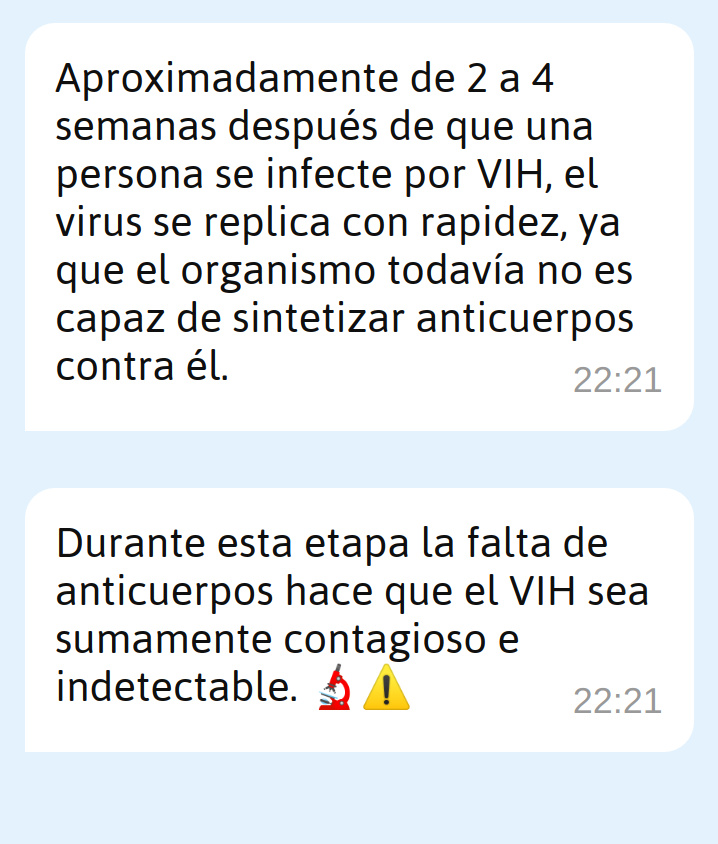
\includegraphics[scale=0.3]{../images/modified_response.png}
\caption{Ejemplo de transformación de una respuesta}
\label{fig:modified response}
\end{figure}

\subsubsection{\textit{Stories}}
Una vez el conjunto de entrenamiento cuenta con la información de los \textit{intents} para identificar las expresiones y sus correspondientes respuestas, es necesario indicarle como debe utilizarlas. Para ello, se incorpora también a los datos de entrenamiento estructuras o patrones de conversación denominadas \textit{stories}. Las historias o \textit{stories} son representaciones de conversaciones entre usuarios y el chatbot. Estos datos utilizan un formato específico en el que la información introducida por el usuario se expresa como \textit{intents} y las respuestas como acciones del asistente \cite{rasaStories}. Por tanto, los \textit{intents} permiten identificar los mensajes de entrada, las respuestas contienen la información, y las \textit{stories} aportan el contexto y la lógica necesaria para responder coherentemente.\\

\begin{verbatim}
  - story: Pregunta por la cura + casos que se han curado + paciente berlin
    steps:
      - intent: cura_vih
      - action: utter_cura_vih
      - intent: faq/casos_cura
      - action: utter_faq
      - intent: faq/paciente_berlin
      - action: utter_faq

  - story: Agradecer + necesita algo más
    steps:
      - intent: agradecer
      - action: utter_no_hay_de_que
      - action: utter_algo_mas
      - intent: afirmar
      - action: utter_ofrecer_ayuda
\end{verbatim}


Tras procesar toda esta información y realizar el entrenamiento, \textit{Rasa} genera un modelo con el cual el asistente es capaz de analizar las preguntas realizadas por los usuarios, asociarlas a uno de los \textit{intents} que ya tenga definidos (en base a una probabilidad) y ofrecer la respuesta correspondiente según le haya sido indicado.\\

\subsection{Servidor (\textit{Backend})}
Una vez el entrenamiento ha finalizado el siguiente paso es hacer accesible el modelo a través de una \textit{API}. Tal y como se ha expuesto en la sección \ref{arquitectura}, \textit{Rasa} pone a disposición los servidores ya integrados dentro del propio \textit{framework} con los que se puede publicar el modelo. Simplemente es necesario configurar los puertos por los cuáles se consumirá el servicio y ejecutar los procesos correspondientes.

\subsection{Vista (\textit{Frontend})}
Debido a su sencillez, la aplicación web se ha construido sin hacer uso de ningún \textit{framework} web, simplemente utilizando \textit{HTML}, \textit{CSS} y \textit{Javascript}. La interfaz sigue los diseños expuestos en la sección \ref{mockups}, implementando un diseño \textit{responsive}. Para ello, se ha utilizado \textit{Flexbox}, un método de diseño unidimensional para colocar elementos en filas o columnas. Cuando el tamaño de pantalla de un dispositivo varía, los distintos elementos se flexionan para llenar el espacio adicional o se encogen para encajar en espacios más pequeños \cite{flexbox}.\\ 

Por otro lado, la mayor parte de lógica de la aplicación ha sido implementada utilizando la librería \textit{Chatbot-Widget} \cite{chatbotwidget}. \textit{Chatbot-Widget} es una librería \textit{opensource} que facilita la implementación y conexión de un chat a la \textit{API REST} del servidor de \textit{Rasa}. Con ella se realizan las diferentes llamadas \textit{HTTP} entre el servidor y la web, enviando los mensajes del usuario y recibiendo las respuestas ofrecidas por el modelo. Además, también facilita la renderización del texto y otros elementos en el chat.\\

Durante el desarrollo, se detectó que la librería presentaba ciertos errores y limitaciones que afectaban al caso de uso específico de VIHrtual-App. Por ello, se realizaron las siguientes modificaciones en la librería:

\begin{itemize}
	\item Corrección de errores en la lógica de llamada-respuesta con el servidor.
	\item Modificación de las funciones de renderización de texto, añadiendo nuevos elementos visuales y soporte para respuestas con múltiples mensajes.
	\item Reescritura de la mayor parte del código CSS utilizando flexbox.
\end{itemize}

Tras su publicación, se corrigieron varios errores que reportaron los usuarios. En la Figura \ref{fig:vistas} se puede observar el resultado final de la aplicación.

\begin{figure}[htbp]
\centering
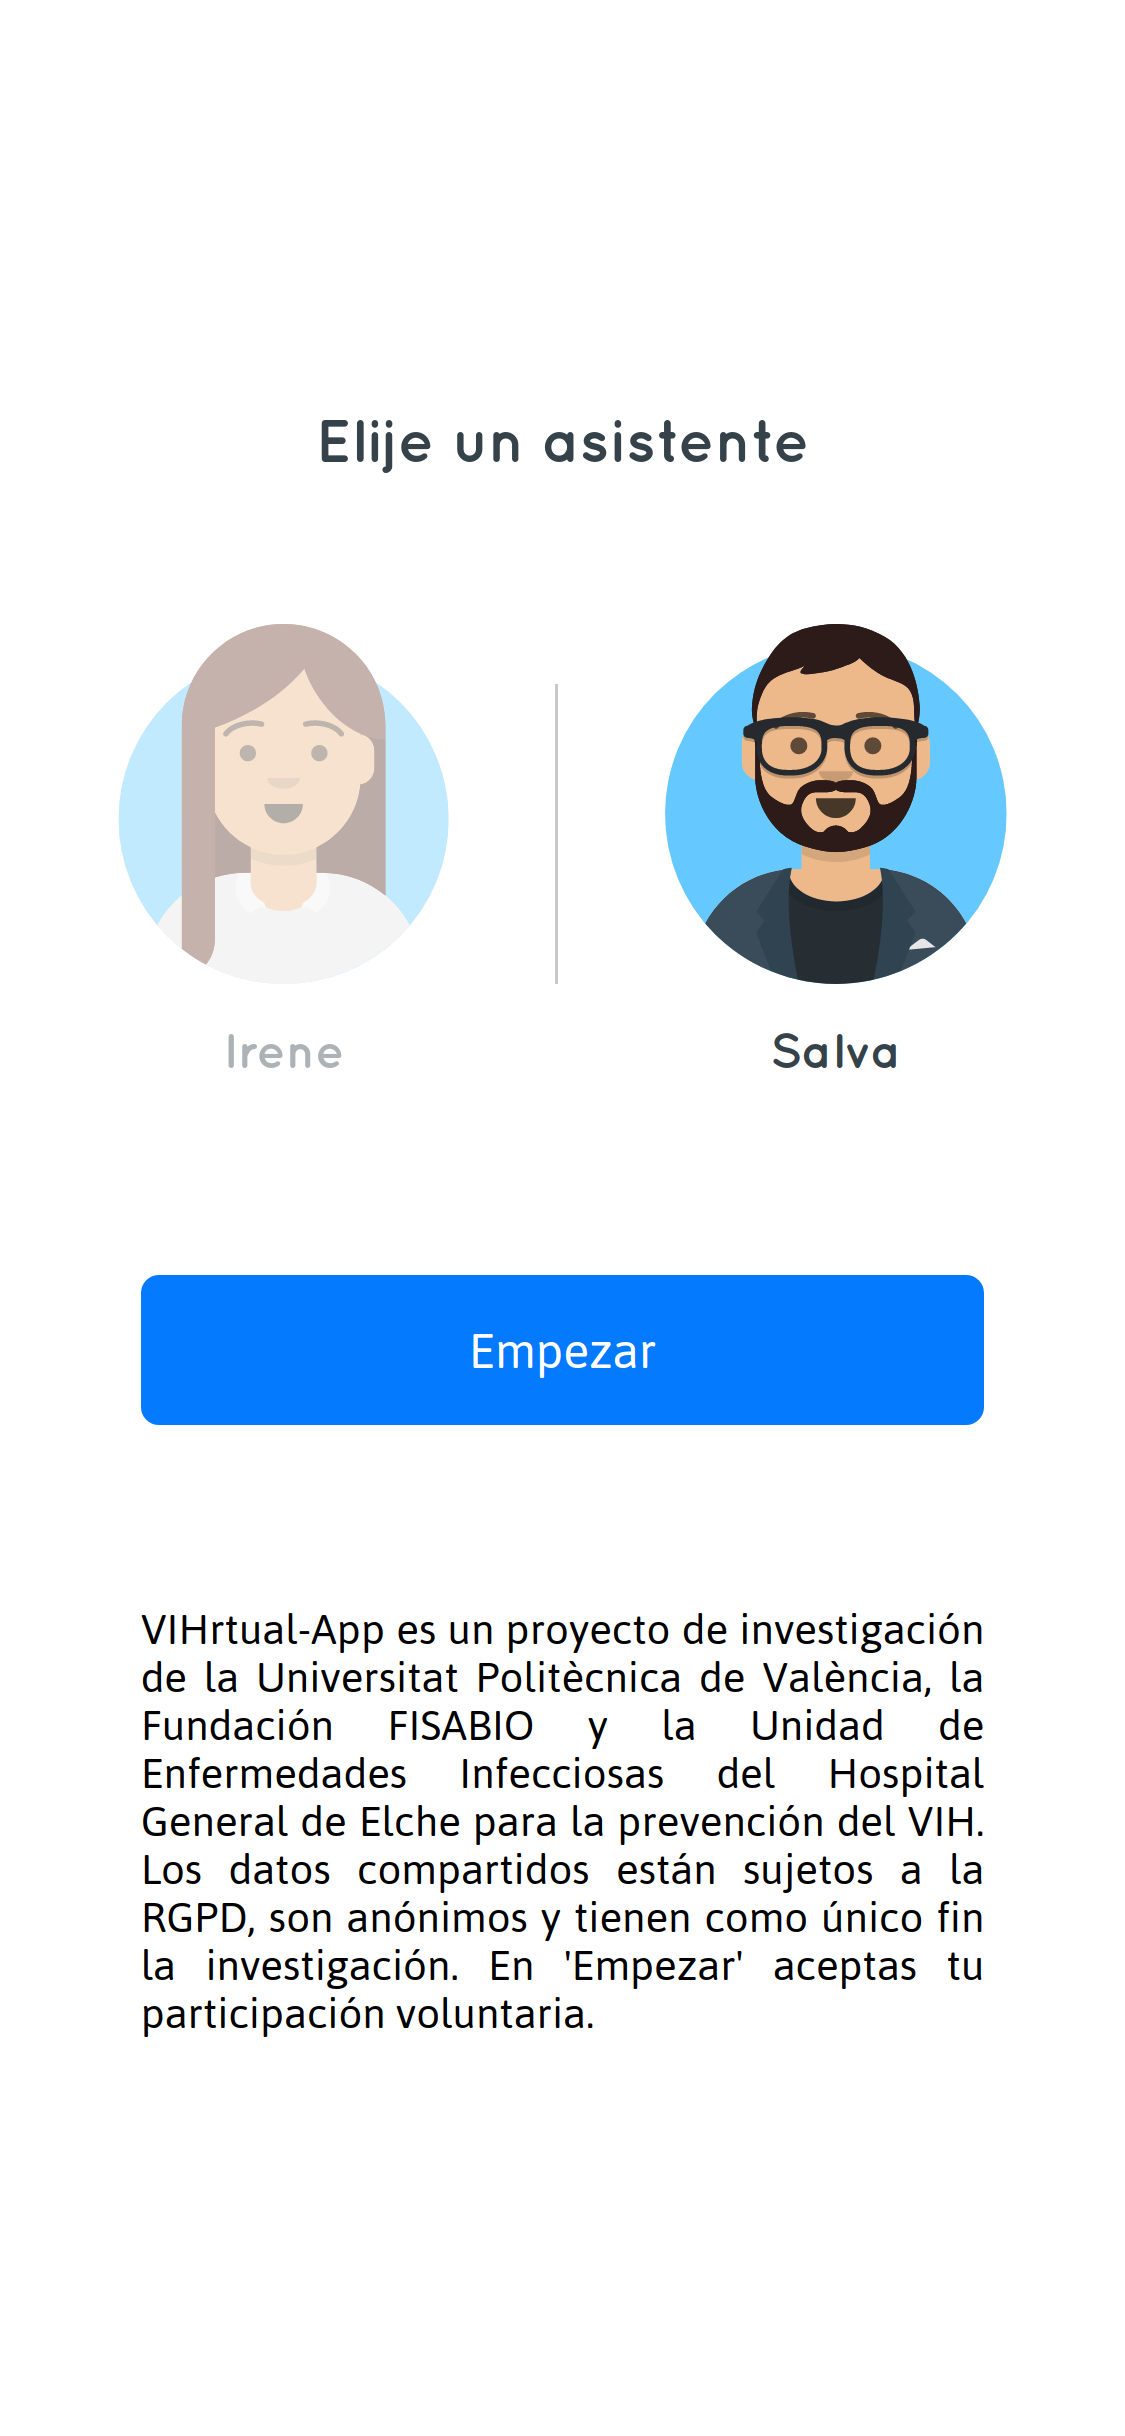
\includegraphics[scale=0.10]{../images/app.png}
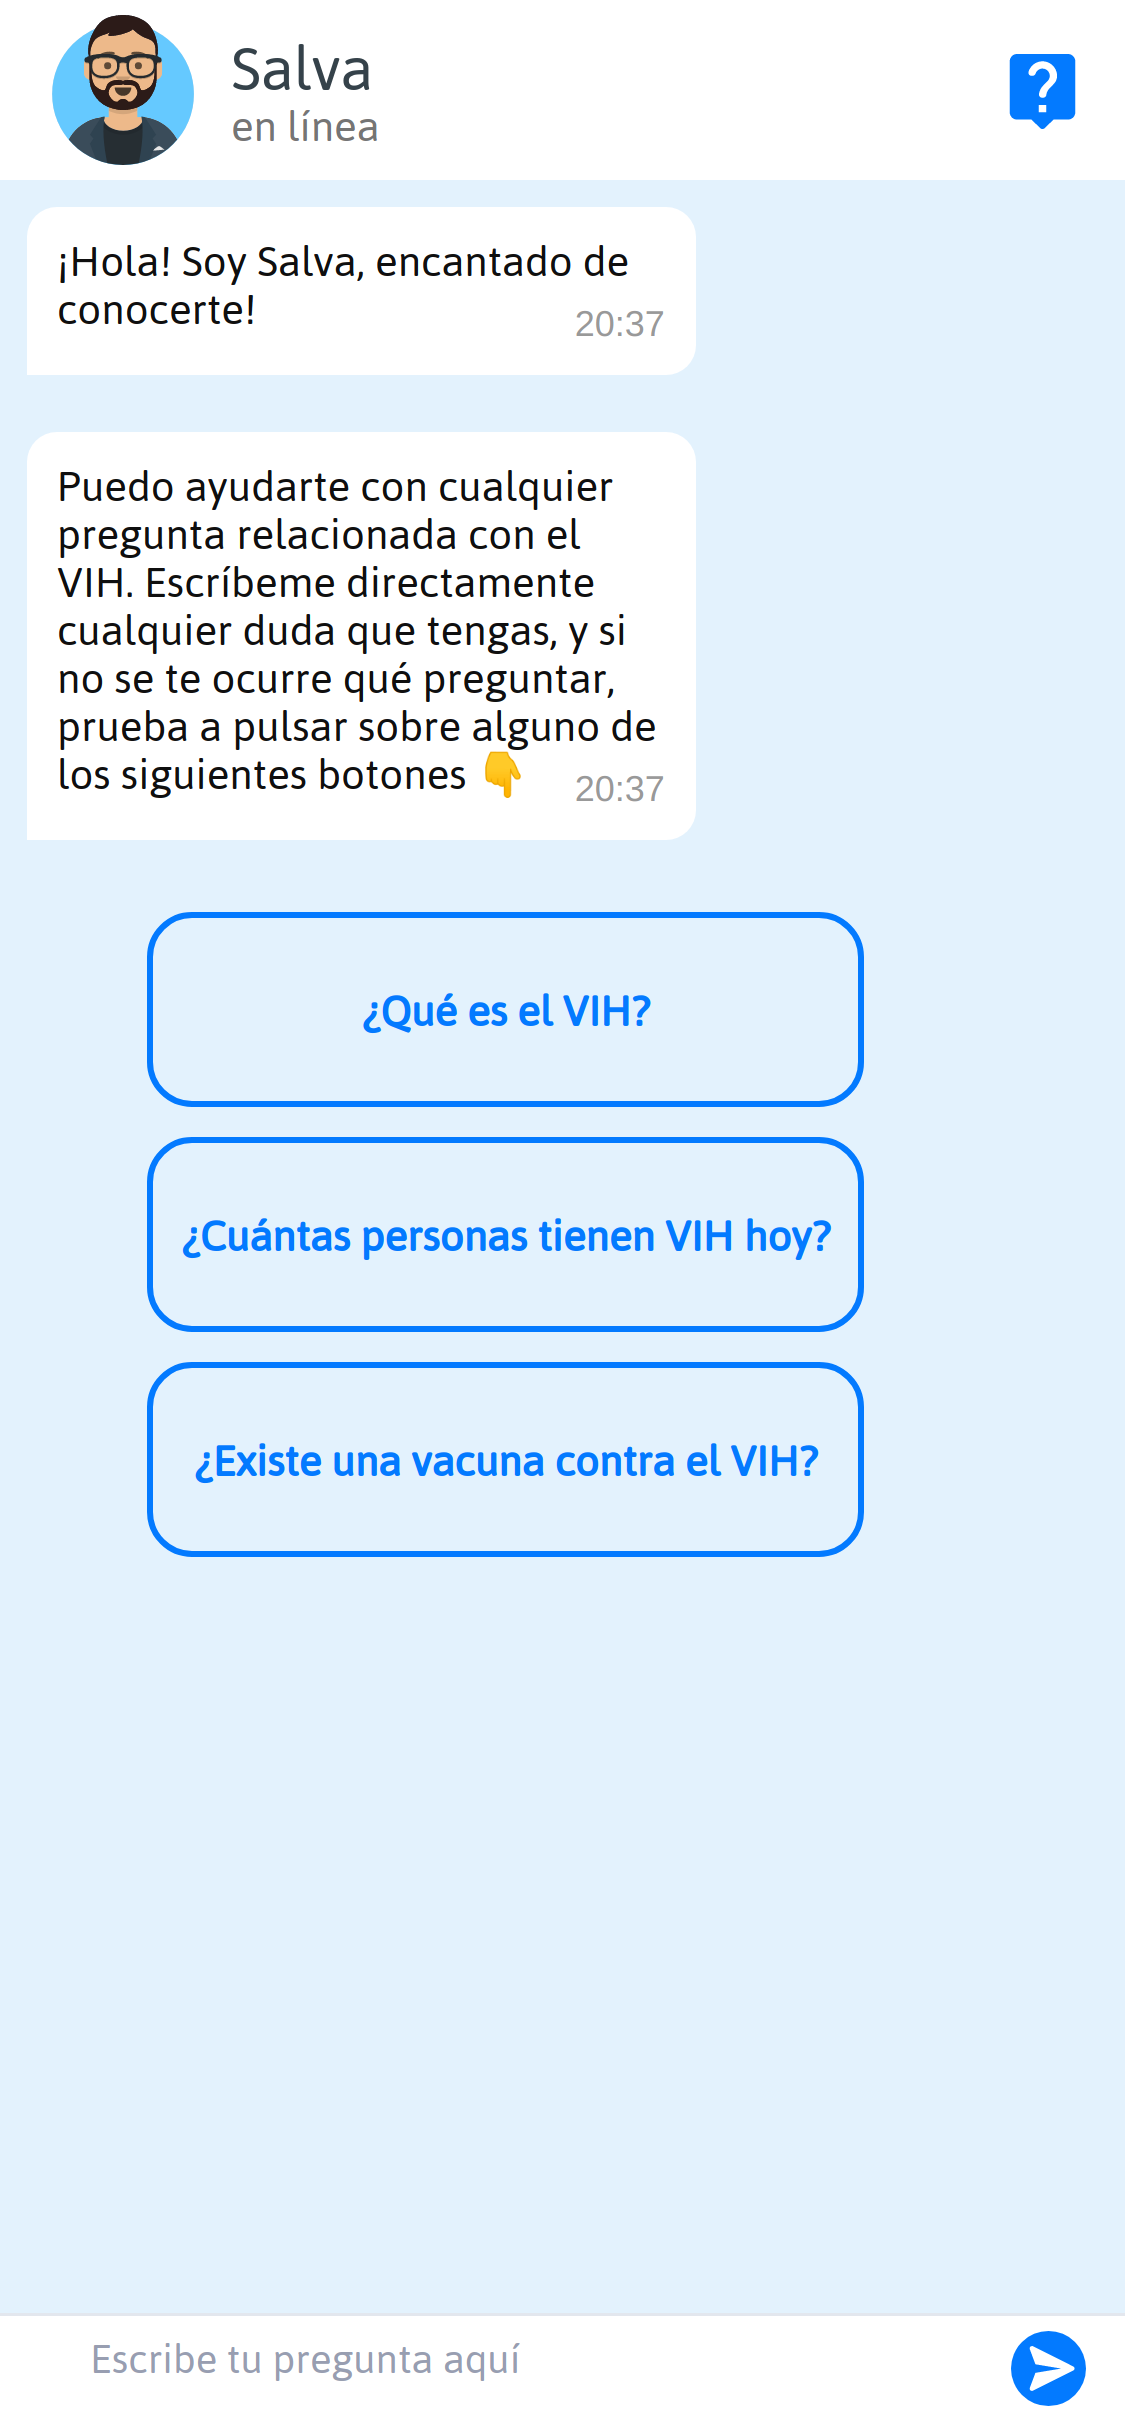
\includegraphics[scale=0.10]{../images/app_2.png}
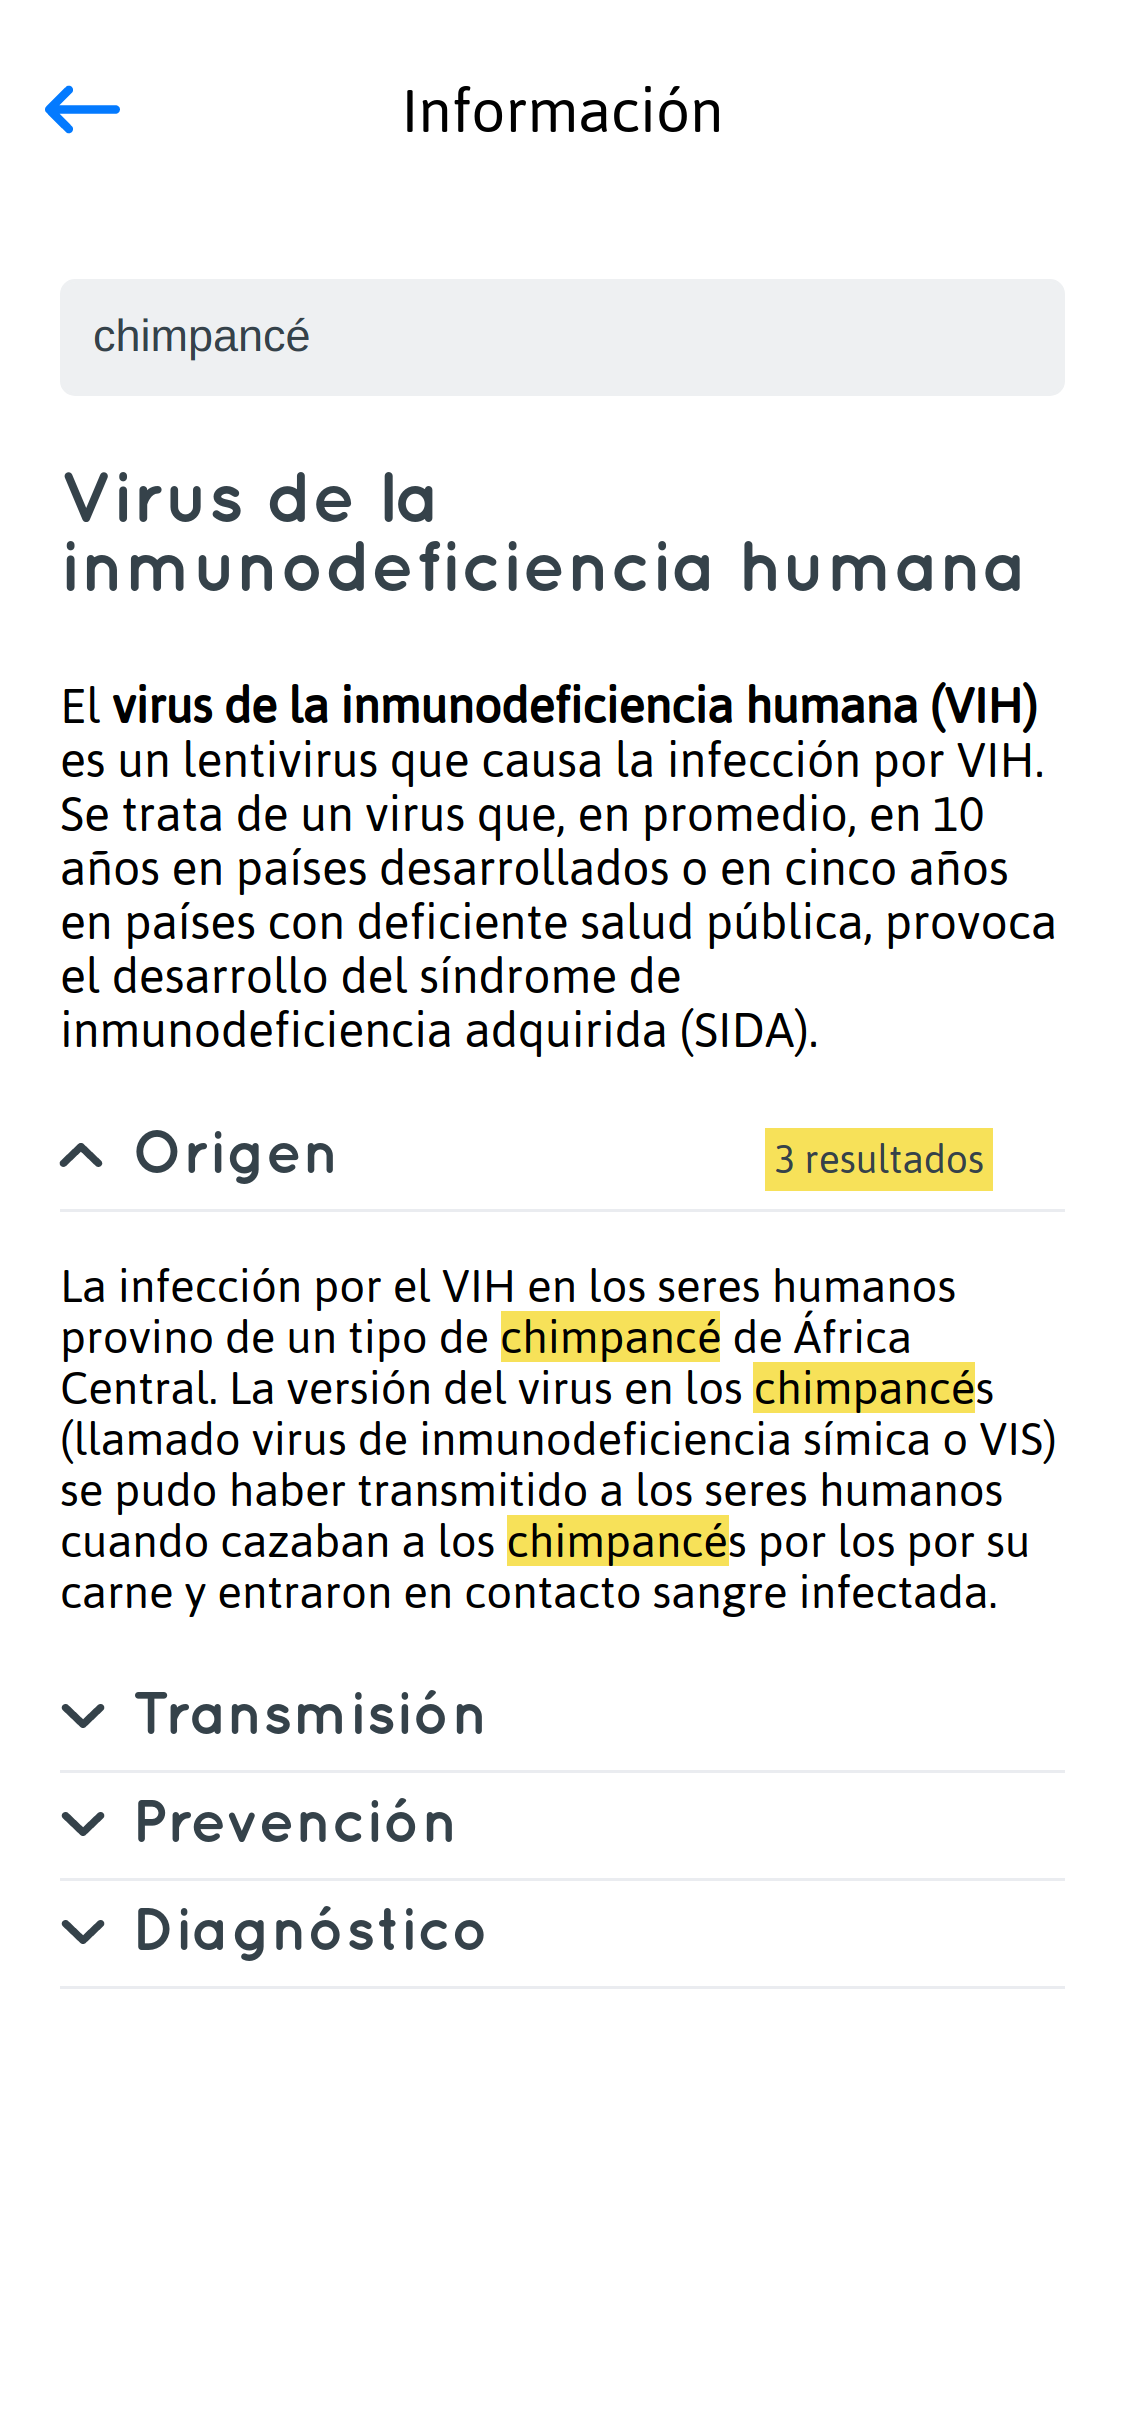
\includegraphics[scale=0.10]{../images/app_3.png}
\caption{Diferentes vistas de la aplicación}
\label{fig:vistas}
\end{figure}


\subsection{Despliegue del prototipo}
\label{despliegue}
Una vez implementados el servidor y el \textit{frontend} web, es necesario publicar una versión de prueba del servicio para poder empezar con la fase de obtención de datos de conversaciones reales. Para ello, la Universitat Politècnica de València pone a disposición del proyecto una maquina virtual con \textit{Ubuntu 18.04} donde poder realizar el despliegue. Mediante acceso \textit{SSH} se instalan todas las librerías necesarias (\textit{Apache}, \textit{Python}, \textit{Rasa}, \textit{Spacy}, etc) y se ponen en marcha tanto la web como el servidor.\\

Una vez el sistema está funcionando, se realiza una pequeña prueba con \textit{Rasa X} para asegurarse que la recogida de datos funciona correctamente. Tras ello, se solicita a la UPV la apertura de los puertos 80, 5055 y 5005 para autorizar el tráfico \textit{HTTP} (ver Figura \ref{fig:ports}), y así, permitir que usuarios externos a la universidad puedan acceder al servicio. De esta manera, el servicio se encuentra disponible desde \textit{http://vihrtualapp.gti-ia.upv.es} y se puede empezar con la recogida de datos.\\

\begin{figure}[htbp]
\centering
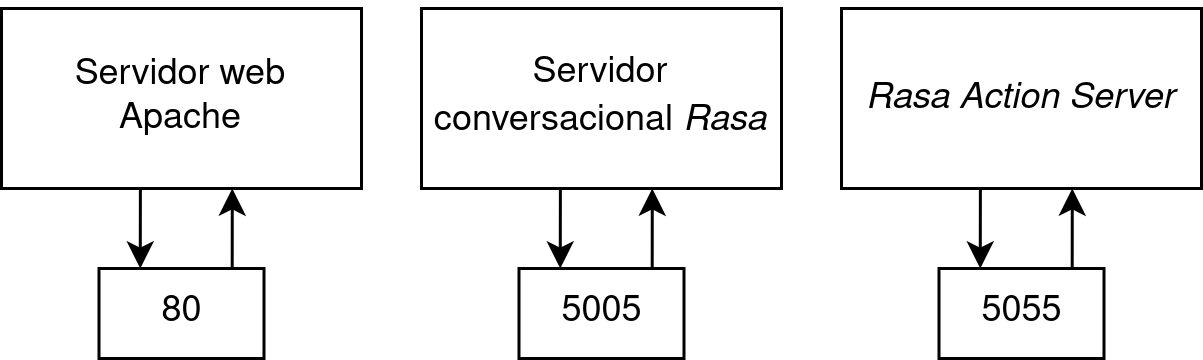
\includegraphics[scale=0.3]{../images/ports.png} 
\caption{Diagrama redirección de puertos y servicios} 
\label{fig:ports}
\end{figure}


\subsection{Desarrollo basado en conversaciones}
\label{cdd}
Uno de los mayores problemas que se suelen presentar durante el desarrollo de un chatbot es que inicialmente, el \textit{dataset} suele estar creado por los desarrolladores, y por tanto, sesgado y alejado de situaciones reales. El desarrollo basado en conversaciones (\textit{Conversation-Driven Development}) es el proceso de escuchar a los usuarios y utilizar esa información para mejorar el asistente \cite{conversationDriven}. Hacer el chatbot robusto puede ser un auténtico reto pues los usuarios siempre introducirán datos que inicialmente no estaban contemplados en el conjunto de entrenamiento. En consecuencia, este enfoque es la mejor manera de solucionar esta problemática, pues toda nueva información se incorpora al \textit{dataset} y así el modelo se nutre de situaciones y expresiones reales. Esta estrategia está especialmente recomendada por los desarrolladores de \textit{Rasa} \cite{bestPracticesNLU}.\\

Tras publicar la primera versión de prueba del chatbot el proyecto se encuentra listo para entrar en esta fase de desarrollo centrada en la recogida de datos. Para ello, durante varias semanas se comparte el chatbot, se revisan las conversaciones obtenidas, y se anotan, clasifican e incorporaran al \textit{dataset} todos los datos recopilados. Tras realizar todos estos cambios sobre el conjunto de entrenamiento se ejecutan los \textit{tests} correspondientes (ver sección \ref{tests}), se corrigen posibles errores y se vuelve a compartir el chatbot para una nueva iteración (ver Figura \ref{fig:cdd}).\\

\begin{figure}[htbp]
\centering
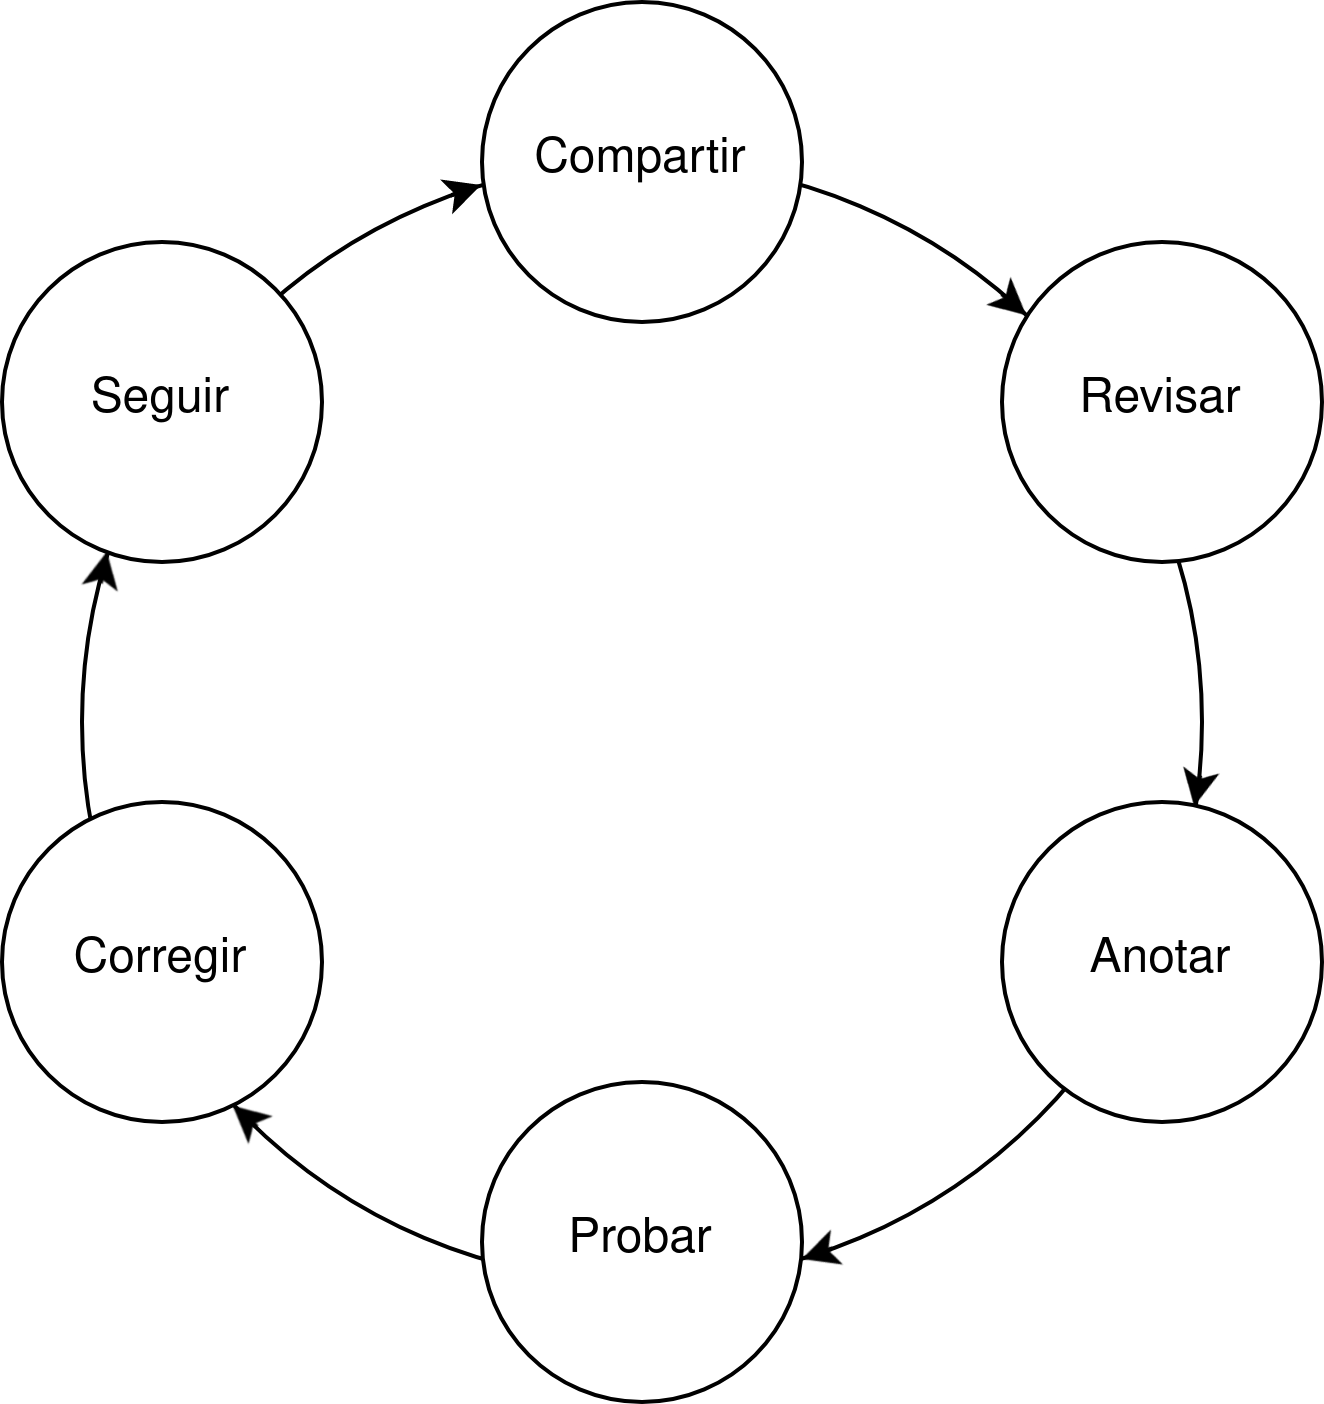
\includegraphics[scale=0.15]{../images/cdd.png} 
\caption{Ciclo del desarrollo basado en conversaciones}
\label{fig:cdd}
\end{figure}

\begin{figure}[htbp]
\centering
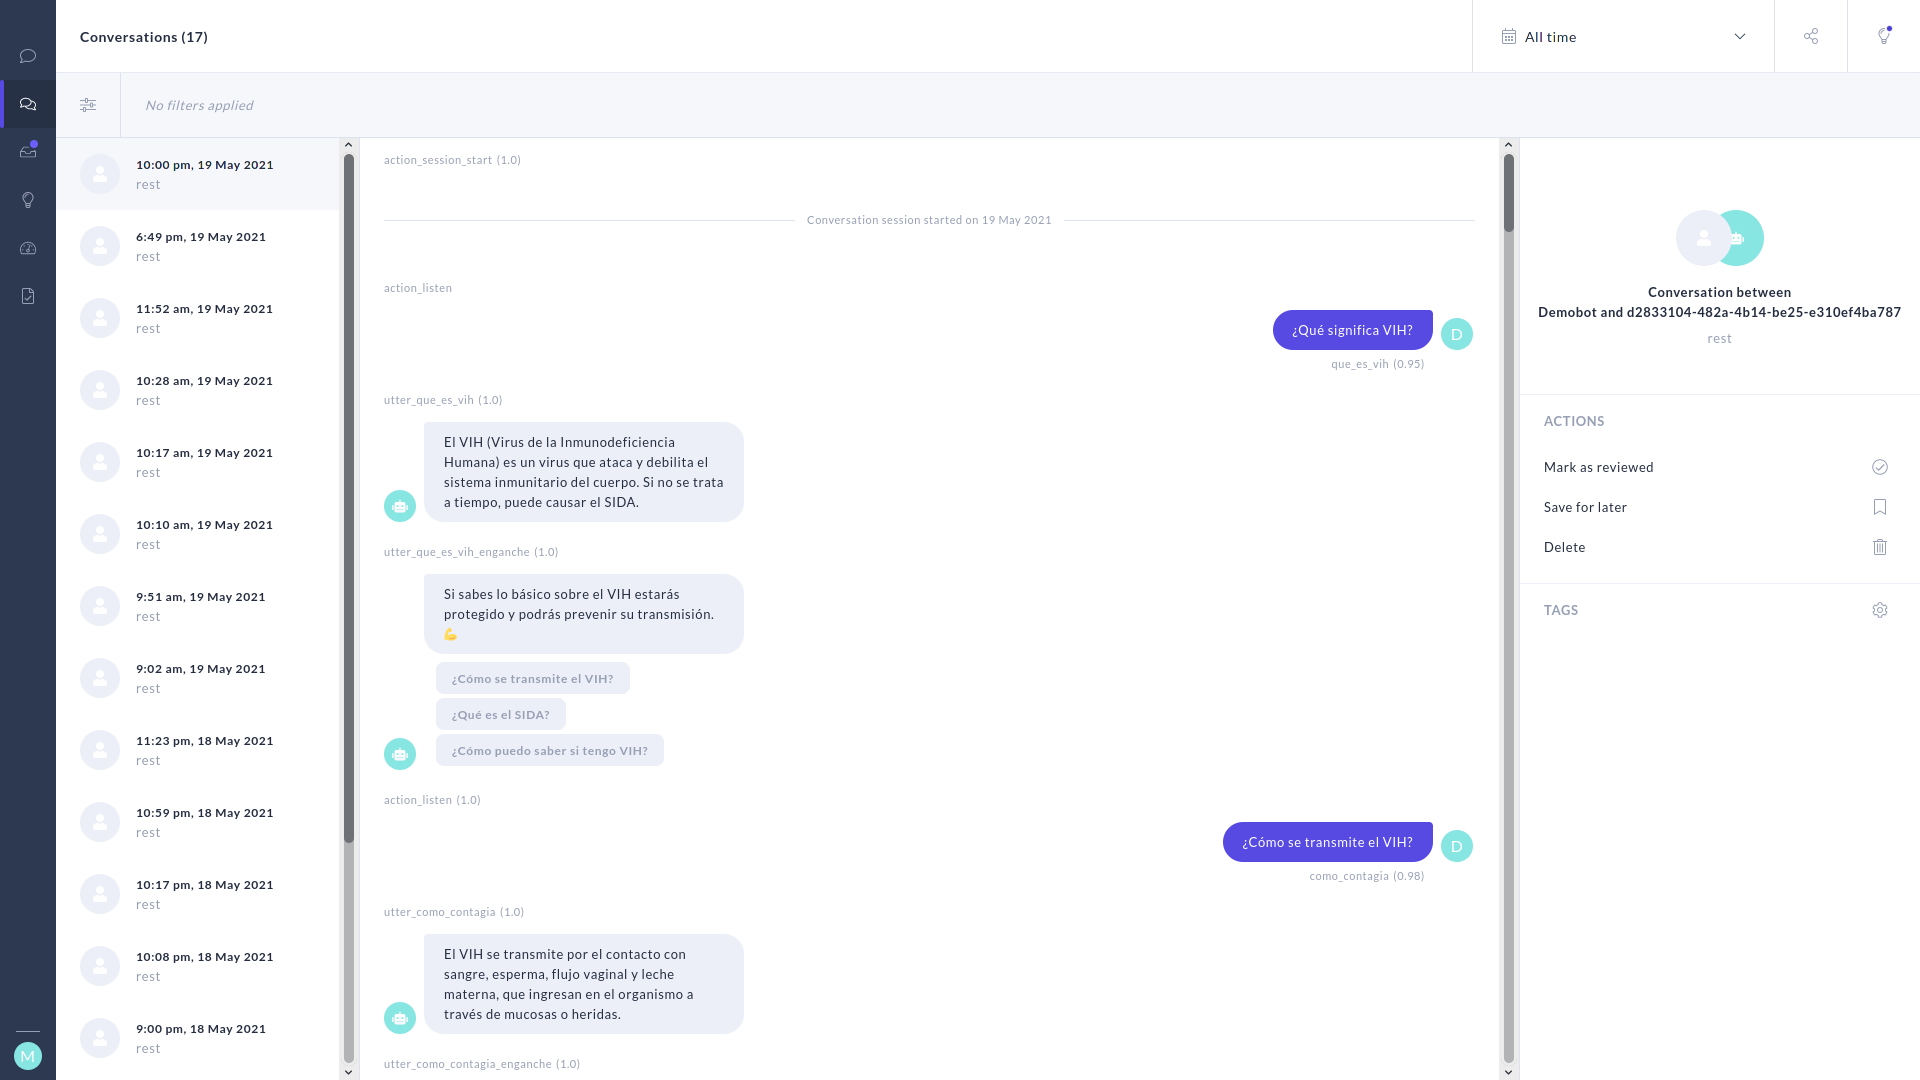
\includegraphics[scale=0.3]{../images/collected_dialogs.png} 
\caption{Ejemplo de una de las conversaciones recogidas}
\label{fig:collected dialogs}
\end{figure}

Para esta nueva fase del desarrollo se hizo uso del servicio \textit{Rasa X}, el cuál facilita la consulta y corrección de todas las conversaciones recogidas. En la Figura \ref{fig:collected dialogs} se puede ver una captura de pantalla del panel de control de \textit{Rasa X}. En la parte izquierda, se pueden consultar todas las conversaciones que el chatbot ha mantenido con los usuarios y, en la derecha, revisar que predicciones de \textit{intents} ha realizado y aplicar las correcciones necesarias. Por otra parte, en la Figura \ref{fig:collected nlu} se puede observar el la herramienta de etiquetado de los datos \textit{NLU} recibidos.\\

Durante todo este proceso se recogieron y analizaron aproximadamente 60 conversaciones de las cuáles se pudo extraer e incorporar a la base de conocimiento la siguiente información:\\

\begin{itemize}
	\item 40 preguntas nuevas (con sus correspondientes respuestas) que inicialmente no estaban previstas.
	\item 232 variantes o expresiones.
\end{itemize}


\begin{figure}[htbp]
\centering
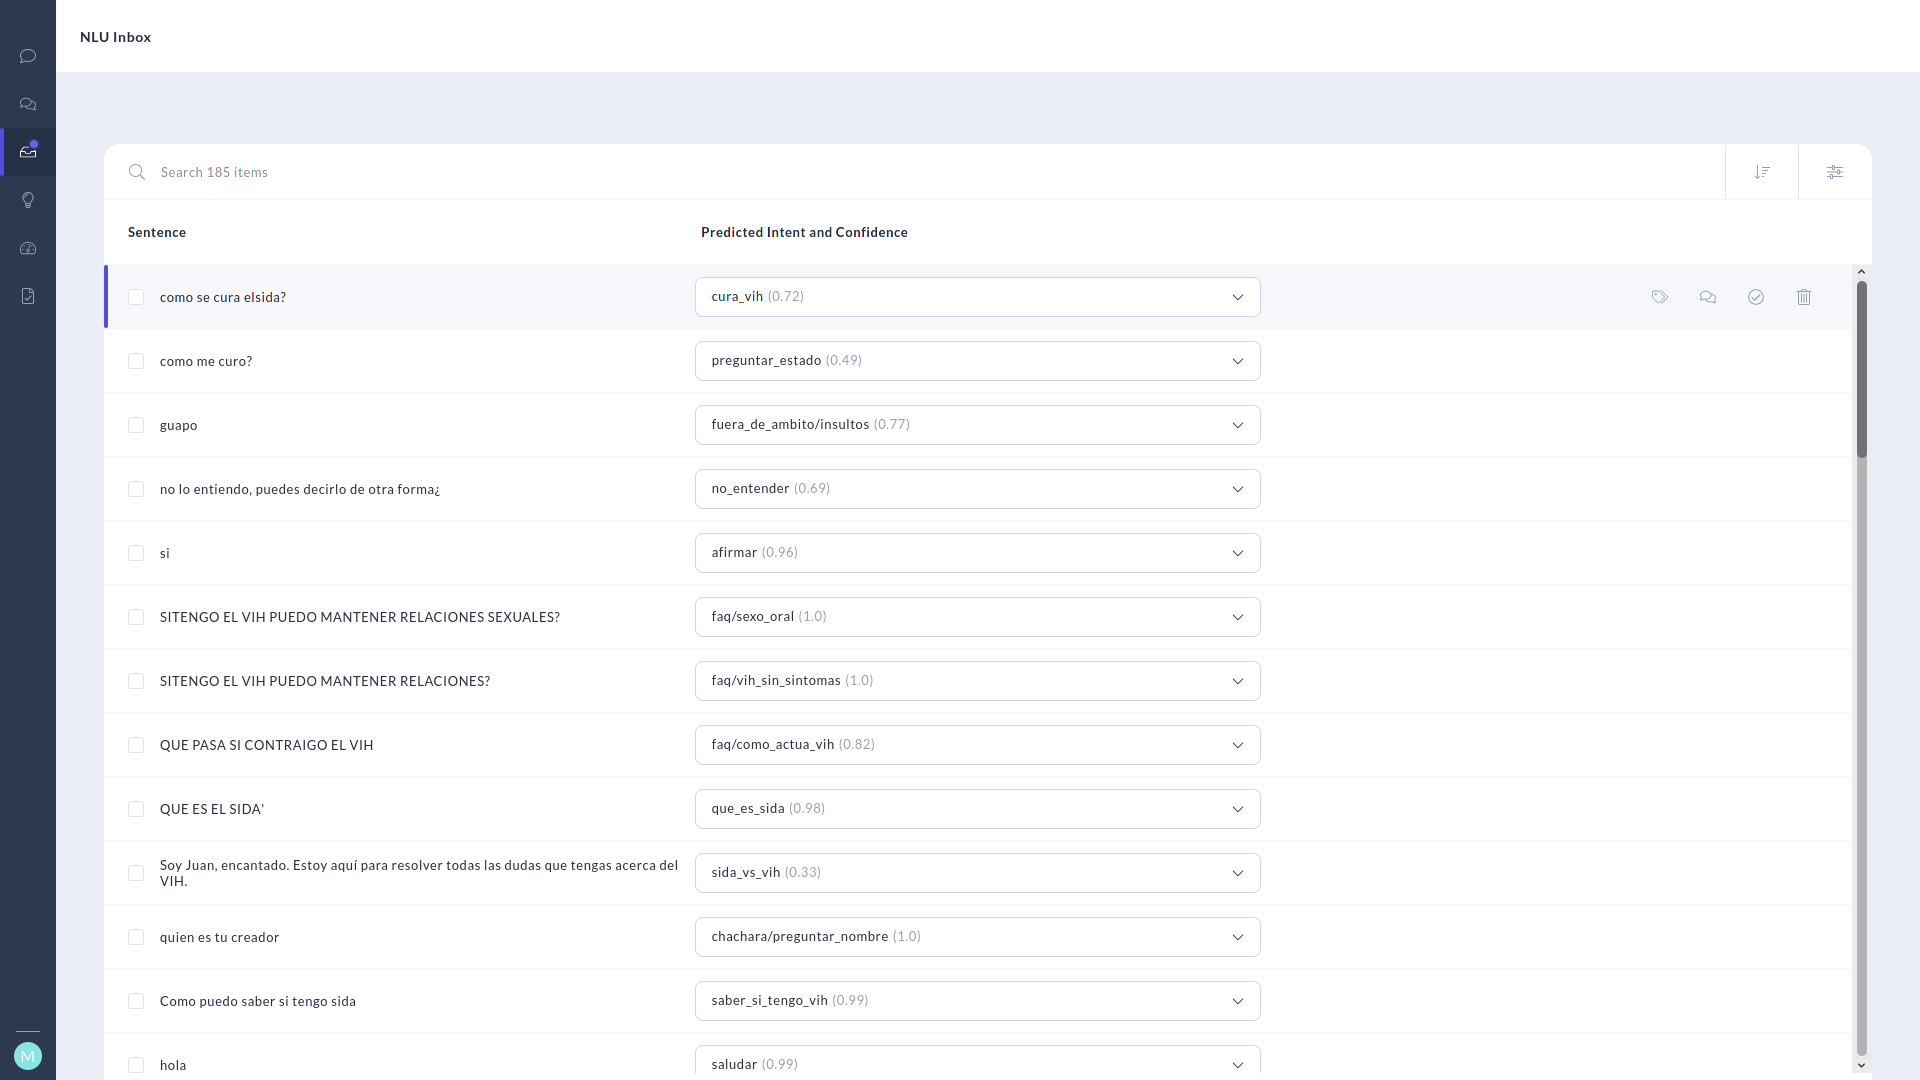
\includegraphics[scale=0.3]{../images/collected_nlu.png} 
\caption{Datos NLU recopilados y su etiquetado}
\label{fig:collected nlu}
\end{figure}

\subsection{Control de daños}
A continuación se describe la implementación de diferentes técnicas utilizadas en \textit{VIHrtual-App} para el control de daños, siguiendo las recomendaciones expuestas en la sección \ref{interaccion}.

\subsubsection{Falta de conocimiento}
Durante el devenir de una conversación es bastante probable que un usuario realice una pregunta que esté fuera del ámbito de conocimiento del chatbot, bien sea por desconocimiento o por poner a prueba el \textit{bot}. Cuando un asistente no responde adecuadamente a este tipo de preguntas puede crear un sentimiento de decepción en el usuario o incluso alentarle a continuar con el comportamiento abusivo \cite{shouldInteract}.\\

Por tanto, todos los casos detectados durante la recogida de información se han recopilado y agrupado en varios \textit{intents} para poder identificar correctamente estas situaciones y ofrecer una respuesta adecuada, intentado siempre reconducir la situación. En la Figura \ref{fig:out1} se puede observar como el asistente reconoce la intención del usuario como fuera del ámbito, le responde disculpándose e indicando que no puede ayudarle en esa tarea y le sugiere algunas preguntas a través de unos botones de respuesta rápida.\\

\begin{figure}[htbp]
\centering
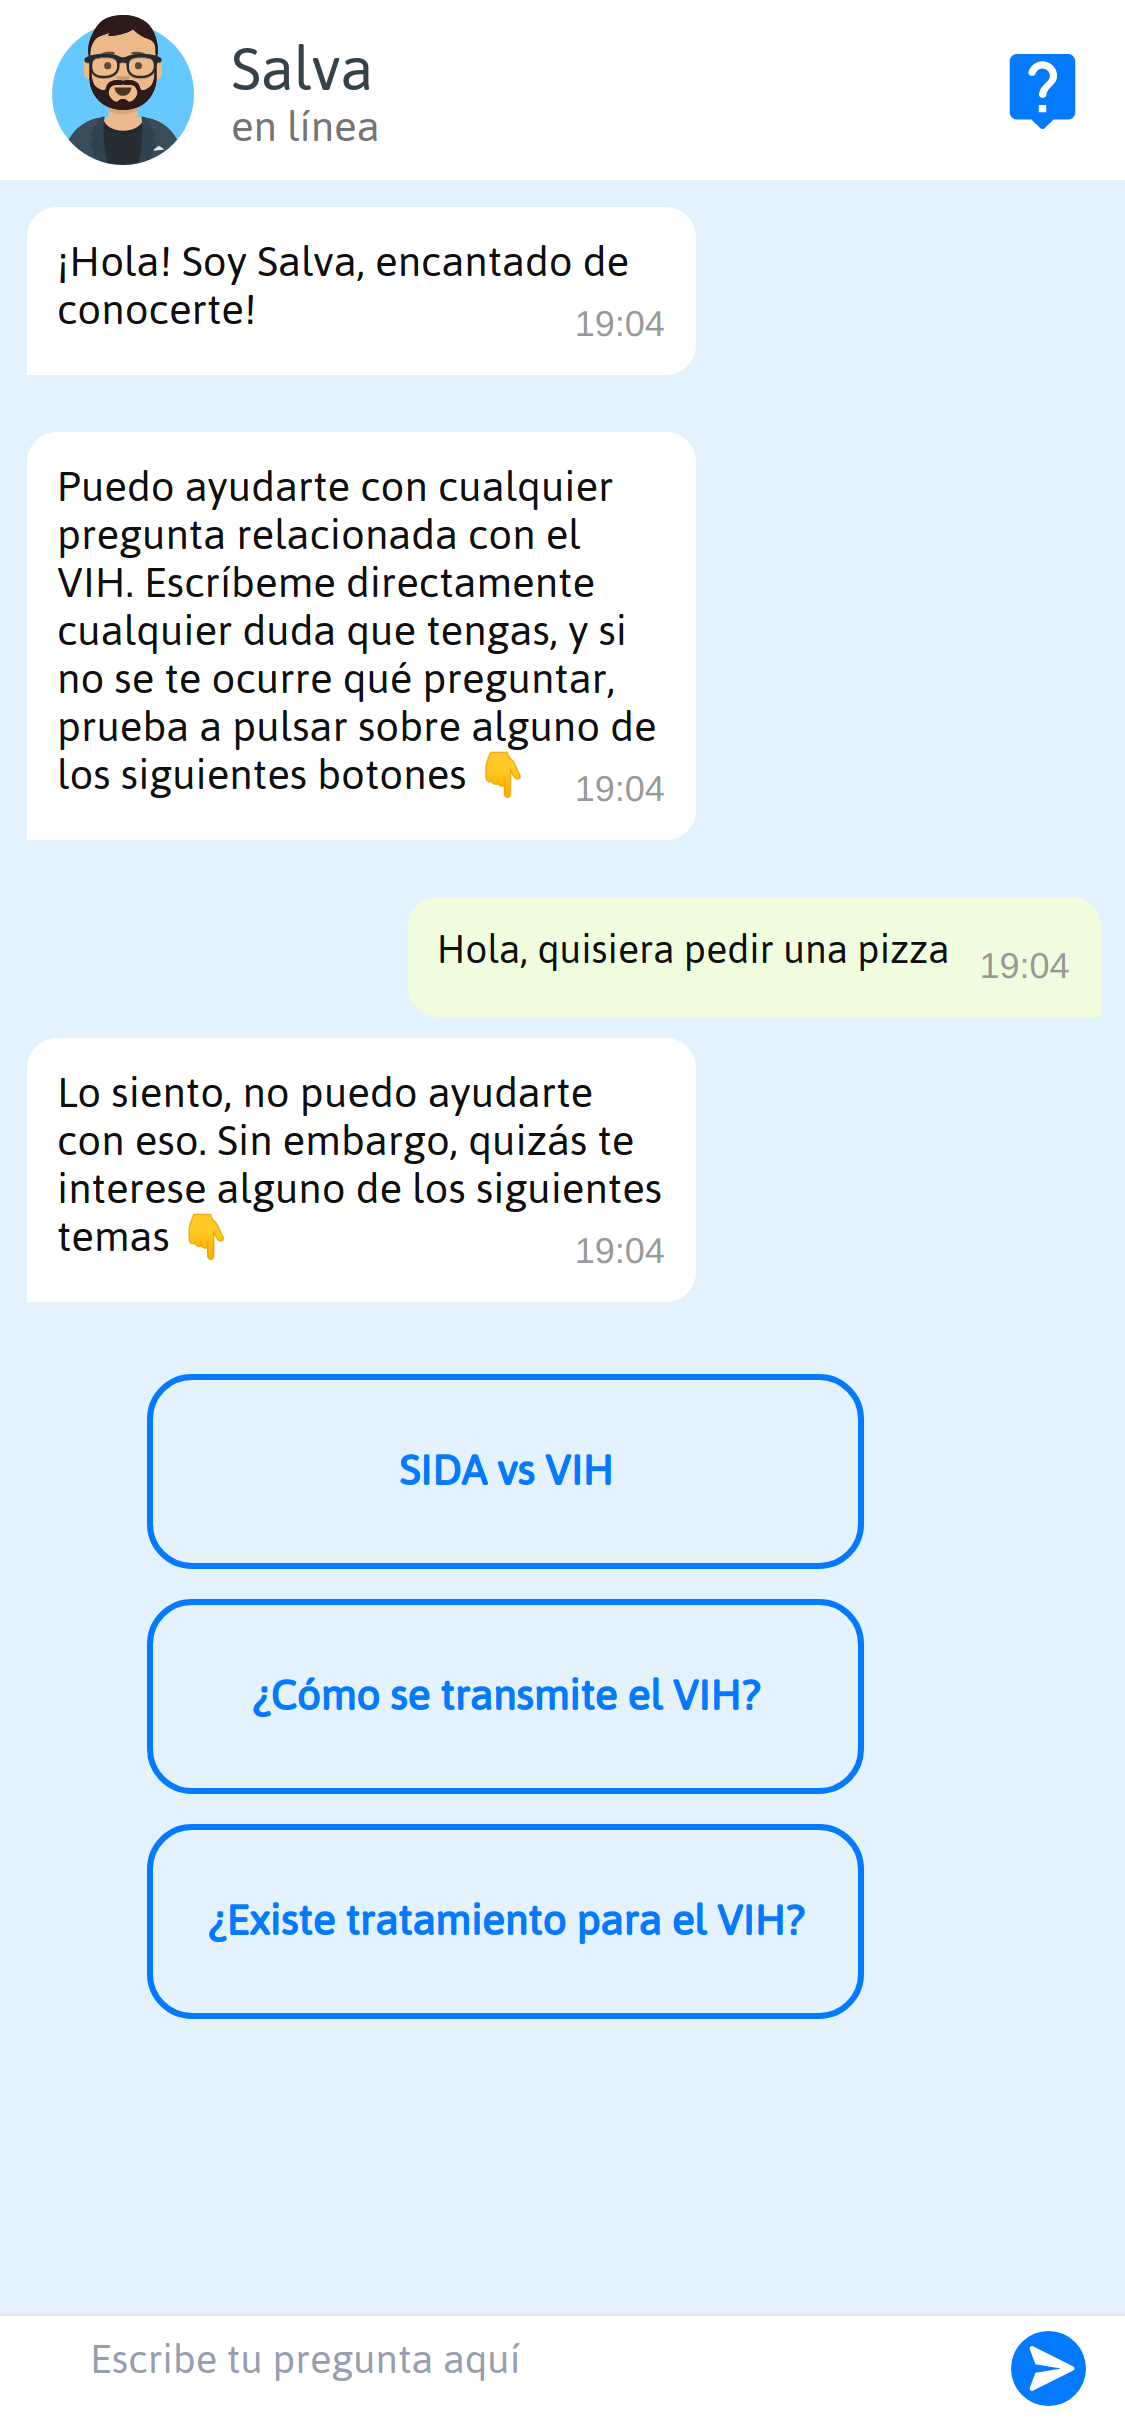
\includegraphics[scale=0.15]{../images/out_of_scope.png}
\caption{Ejemplo de manejo de mensajes fuera de ámbito}
\label{fig:out1}
\end{figure}

\subsubsection{Conductas abusivas}
Por otra arte, los chatbots suelen ser más objeto de insultos y vejaciones de lo que un humano en una conversación real seria \cite{shouldInteract}. En este caso, la estrategia es idéntica, se recogen los datos necesarios para reconocer las situaciones y se responde para evitar que el usuario continue con su comportamiento. En la Figura \ref{fig:recover} se puede ver como responde el \textit{bot} ante un usuario poco amigable.\\

\subsubsection{\textit{Fallback}}
Por último, y como último recurso, cuando el chabot no es capaz de identificar con suficiente confianza un \textit{intent}, muestra un mensaje disculpándose y preguntando amablemente si el usuario es capaz de reformular la pregunta. De esta manera, se intenta forzar al usuario a expresar su intención en otras palabras para poder tener una nueva oportunidad de reconocimiento. En la figura \ref{fig:recover} se puede observar un caso como el expuesto donde \textit{bot} es capaz de recuperase ante un fallo inicial.\\

\begin{figure}[htbp]
\centering
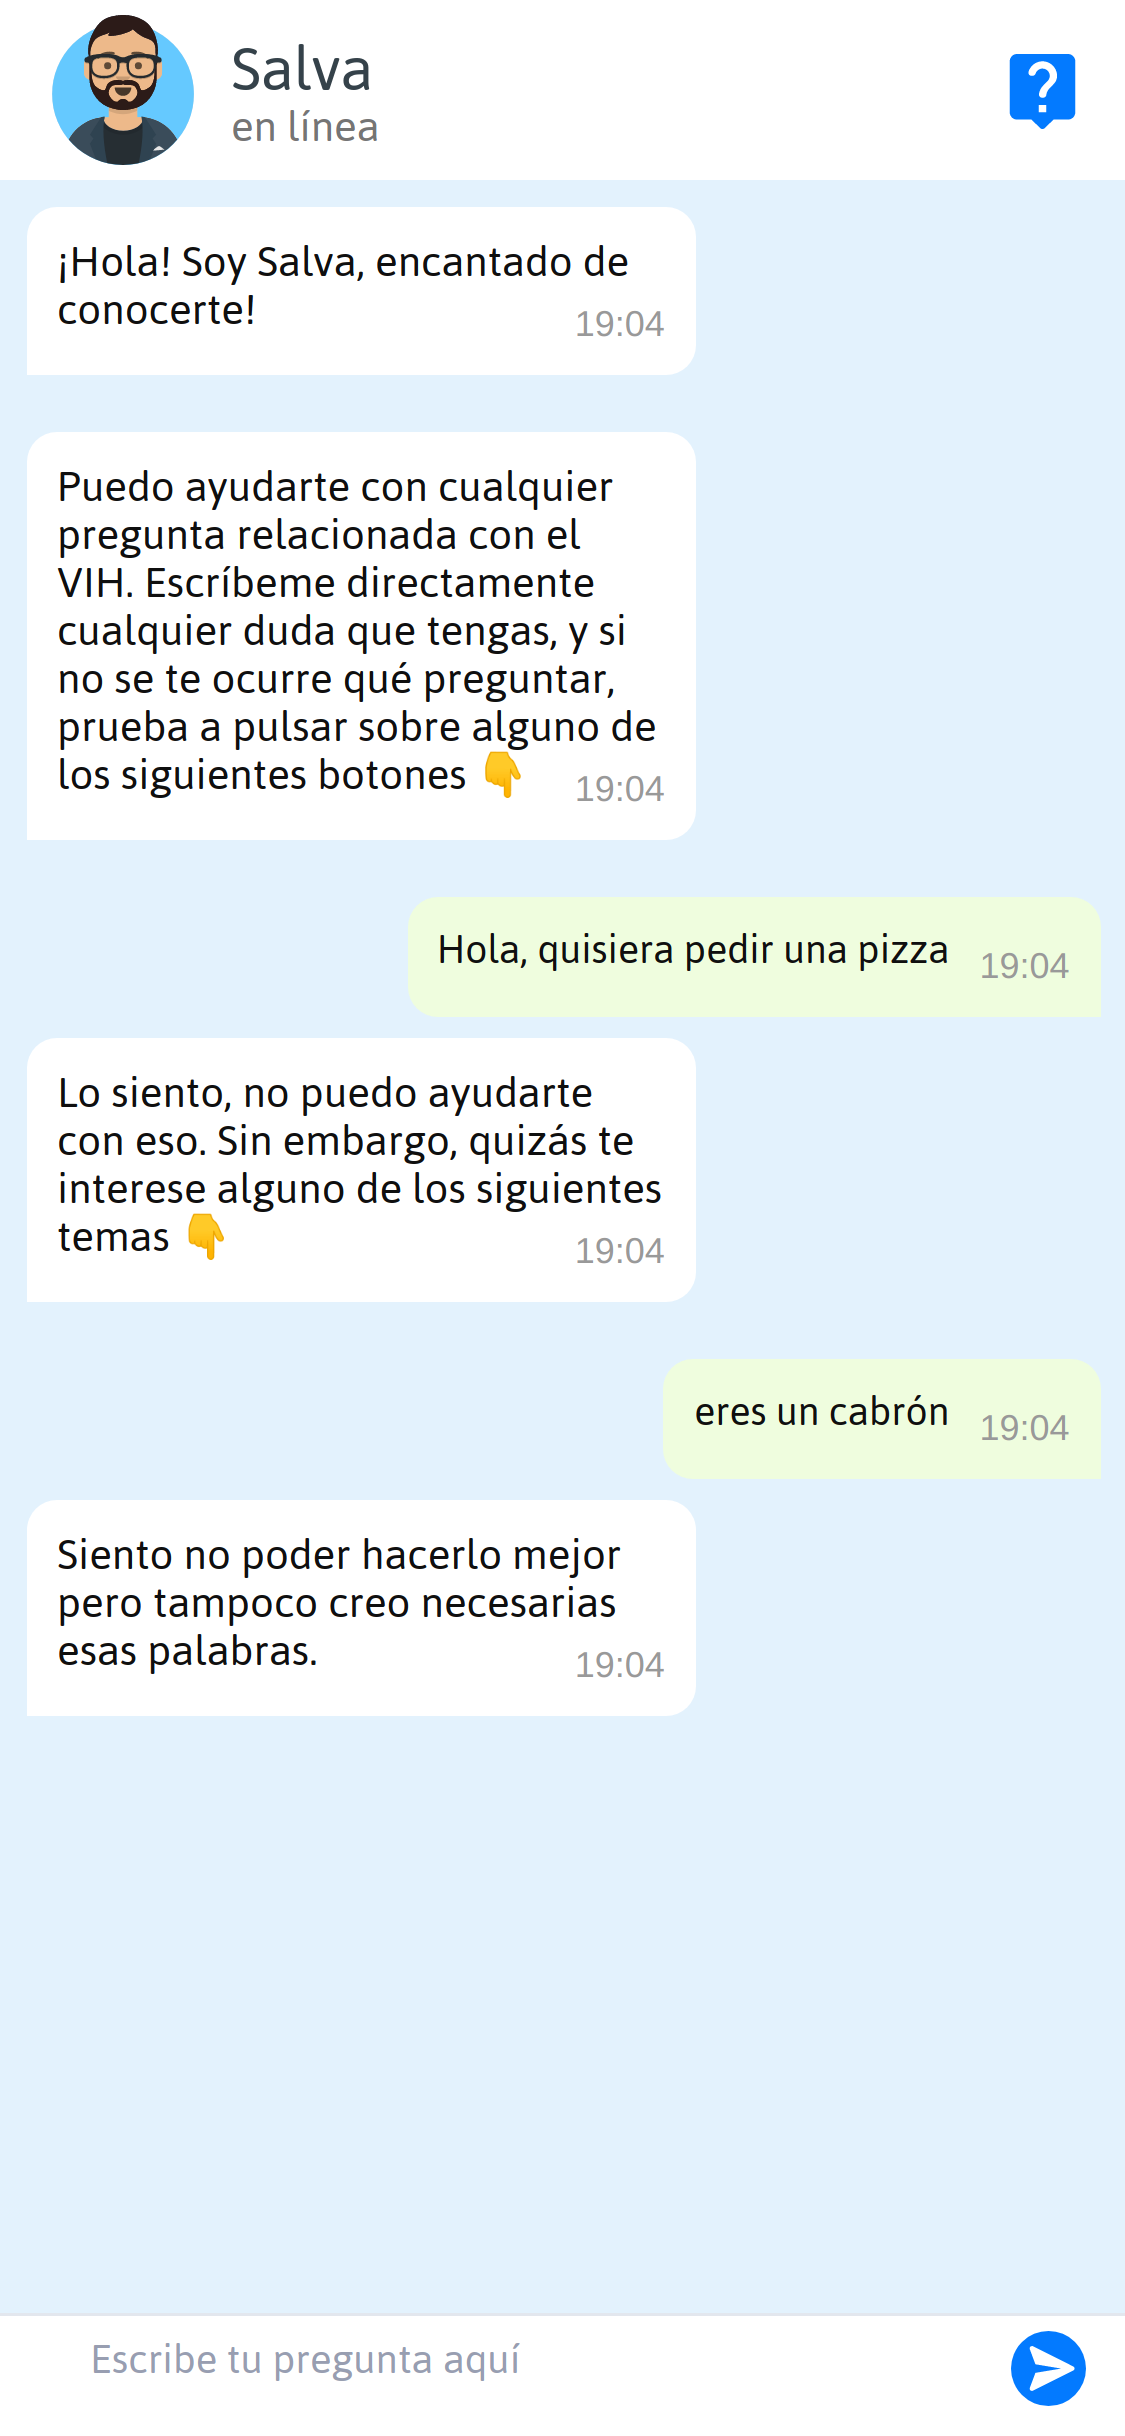
\includegraphics[scale=0.15]{../images/out_of_scope_2.png}
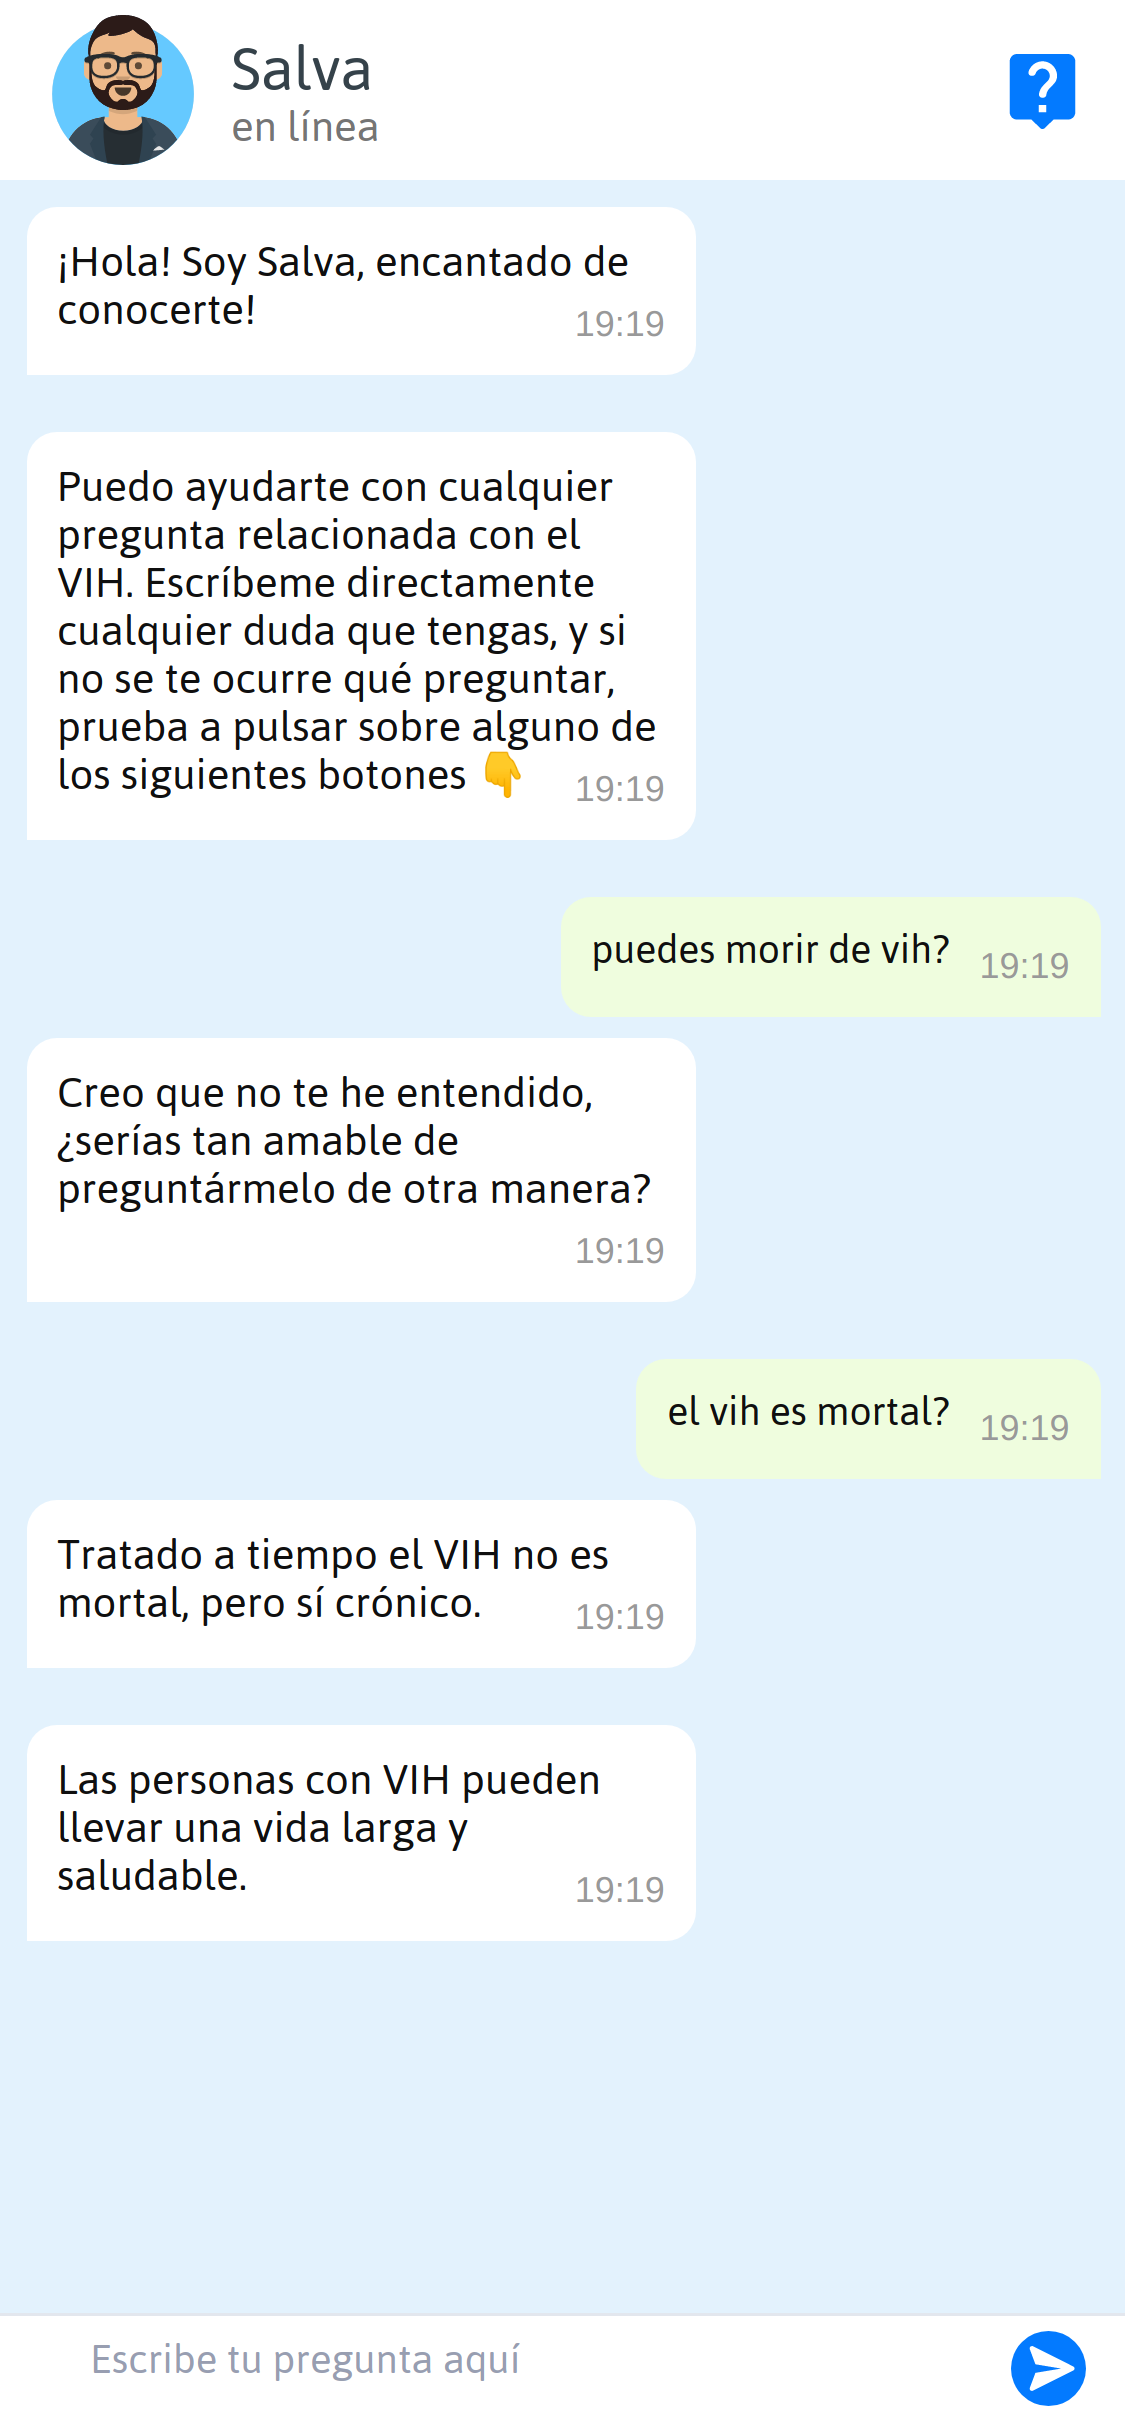
\includegraphics[scale=0.15]{../images/recover.png}
\caption{Ejemplo de recuperación ante insultos y identificación de \textit{intent}}
\label{fig:recover}
\end{figure}

\subsection{Tests}
\label{tests}
Tal y como se ha expuesto anteriormente en la sección \ref{cdd}, durante el desarrollo basado en conversaciones una parte importante del ciclo cosiste en realizar frecuentemente \textit{tests} automáticos. Tradicionalmente, en el mundo del \textit{software} se entiende por \textit{test} una prueba que verifica que una función devuelve el valor esperado. En \textit{Rasa}, los \textit{test} miden si los modelos generados hacen las predicciones correctas \cite{rasaTests}.\\

A medida que el desarrollo avanza, se van incluyendo cada vez más \textit{stories}. Por ello, para evitar inconsistencias es importante asegurarse de que con cada nueva funcionalidad añadida, el modelo continua comportándose como esperamos. Para este cometido \textit{Rasa} ofrece un formato específico con el que escribir tests y así poder asegurarse periódicamente que el modelo no presenta errores.\\

Las \textit{test stories} son un formato modificado de \textit{stories} que incluyen también los mensajes de los usuarios. De esta manera, los tests aseguran que, ante un determinado \textit{input}, el modelo se comportará de la manera esperada. Siguiendo con el ejemplo visto anteriormente, para la \textit{story} donde el usuario le da las gracias al chatbot y este le pregunta si necesita algo más, se obtienen el siguiente test.\\

\begin{verbatim}
  - story: Agradecer + necesita algo más
    steps:
    - intent: agradecer
      user: |-
        muchas gracias!
    - action: utter_no_hay_de_que
    - action: utter_algo_mas
    - intent: afirmar
      user: |-
        siii
    - action: utter_ofrecer_ayuda
\end{verbatim}

La estrategia seguida para la implementación de los tests en VIHrtual-App ha sido implementar, para cada \textit{story}, un test. De esta manera, cada nuevo patrón de conversación introducido en el modelo dispone de su correspondiente prueba. Esto ha permitido evitar regresiones durante todo el desarrollo.\\

\subsection{Distribución}
Adicionalmente, y una vez el chatbot sea considerado estable, se publicará para aquellos usuarios que lo deseen una aplicación web empaquetada para \textit{Android} y para \textit{iOS}. Esto permitirá que aquellos usuarios interesados puedan instalar el servicio desde las tiendas de aplicaciones habituales en sus dispositivos móviles.\\

Aunque aún no está disponible al público, este empaquetado se ha realizado utilizando \textit{Capacitor} \cite{capacitor}, una herramienta que permite crear binarios para plataformas móviles.\\


